\section{Problem Formulation}
\label{sec:problemformulation}

In this section, we analyze the wireless spectral resources allocation in access multiple tiers of wireless
multihop access netowrks. 
Then, we focus on the two network access and backhaul tiers and the impacts between each tier. 
Further, we introduce and analyze wireless access networks 
which jointly use WiFi and white space 
frequencies in a wireless multihop network. 
%We propose two models to discuss the influences of WiFi and white space frequencies in wireless mesh 
%network design in access and backhaul tiers. 


\subsection{Wired and Wireless Connections}

% Wireless network functioins, tiers
The key objective of network deployment is to serve the traffic demand of the users.
Largescale wireless access networks deployed in municipal districts, neighborhoods, school campuses, and office buildings 
can have two network tiers: {\it (i)} an access tier, where 
users directly communicate to access points, and {\it (ii)} a multihop wireless backhaul tier for connecting 
all access points to the Internet through gateway nodes. 


% Introduce the two tiers with the wireless and wired connections, gateways/etc.
\textbf{Access Tier.} 
% Network Constraint
An access point should ideally provide network capacity which is at least as high as the user traffic demand of the service 
area. The deployment of the access tier is subject to the coverage constraint of a given area and the capacity 
constraint of the users in the area. The coverage constraint is defined with respect to the ability of 
users to connect to access points within their service area quantified by $R_p$. The capacity constraint is defined with 
respect to the ability of a network to serve the traffic demand of users quantified by $R_{QoS}$. 

\textbf{Backhaul Tier.} 
Access points may communicate directly to one another to form a wireless backhaul tier which forwards traffic to and from 
gateway points to reach the wired or wireless Internet entry points. 

%Spatial reuse allows improved 
%capacity but increases the cost of deploying a large-scale network by increasing the total number of access points 
%required. 

Both wired and wireless connections can provide Internet entry points for the access and backhaul tiers.
Wired connections offer stable and qualified services with high deployment cost. 
While wireless connections offer convenient and affordable services with low deployment cost. 
Wireless is an ideal option to deploy network with low cost.
However, the spectral resources are limited in nature and restricted by governmental policies. 
With certain amount of spectral resources, there is a competition between the two tiers for resources allocation.
Human factor works have shown the users prefer wireless connections to wired connections for their 
devices in the access tier~\cite{lu2003technology}. To improve the user experience, the access tier is 
given priority with the spectral resources.


% Here
% Wired
Thus, as the user population density increase, the access tier will take more spectral resources which reduce
the resources left for backhaul tier.
We have a rough analysis of wireless network capacity. 
We first allocate the spectral resource to the access 
tier according to the traffic demand generated by the users. 
To simply the analysis we assume a fully spatial reuse in backhaul 
tier as all the spectral resources allocated to the tier can be reused through power control.
We assume there are 10 non-overlapping channels in a 4x4 unit grid area, 30\% of the residents wil use the service. 
An individual user would have a 2 Mbps traffic demand on average. Each channel has 600 Mbps capacity.
% Modify
The access tier requests 4 channels in low population density and scales up by 4 as the population density increase in 
this example.
As shown in Fig.~\ref{fig:spectral_allocation}, the maximum total traffic served of the network increase with the traffic 
demand which is proportional to the user population density at the beginning. 
As the population density increase, the total traffic demand aggregated to the backhaul tier reach the 
capacity of the assigned spectral resources.
We obesrve with more wired gateways, the backhaul serves more traffic demand in the example.
When the access tier scales up the spectral resources request, 
the total traffic served decrease sharply in the 3 curves due to the backhaul tier wireless capacity reduction.

\begin{figure}
\vspace{-0.0in}
\centering
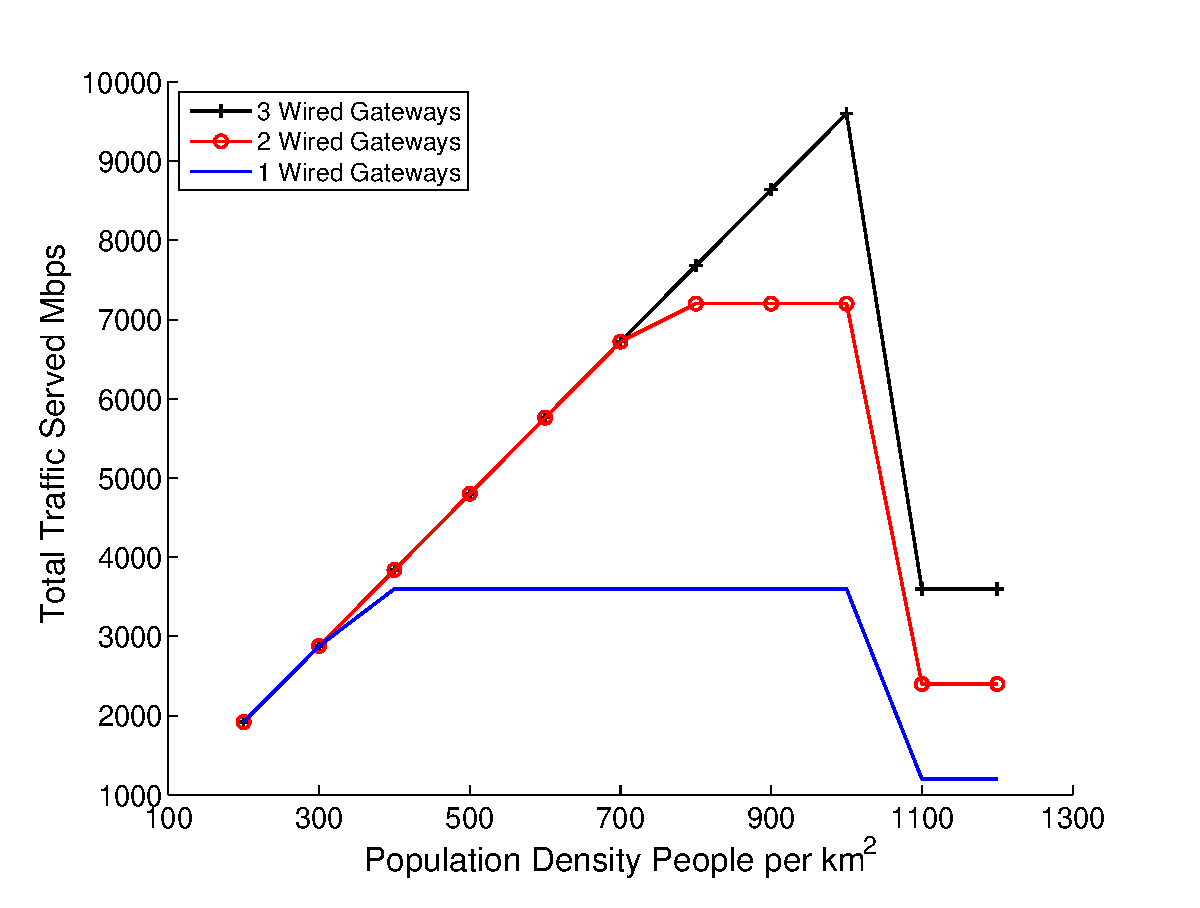
\includegraphics[width=64mm]{figures/spectral_allocation}
\vspace{-0.1in}
\caption{Total Traffic Served Traffic with Wired Gateways}
\label{fig:spectral_allocation}
\vspace{-0.3in}
\end{figure}

% what the problem and how to solve the, then connect whitespaces
In the access tier, the network design focuses more on reducing the deployment cost with prior spectral resources allocation.
While in dense populated area, the capacity of spectral resources is not able to fulfill the backhaul requirement. 
At the same time, there are more infrastructures available for wired gateways increasing the capacity of backhaul tier. 
Thus, the backhaul tier could increase either the wired gateway numbers or channel efficiency to meet the traffic demand 
requirements.
The questions of network deployment in wireless
are to reduce the access tier cost and increase the backhaul channel efficiency.
Prior work of wireless networks focused on improving the capacity 
by reducing the interference among the links~\cite{si2010overview,doraghinejad2014channel}. 
However, many of these works assume a uniform propagation ability of the multiple channels used in the deployment.~\cite{doraghinejad2014channel}. 
In this work, we study the non-uniform propagation multiband scenarios of wireless network design in access tier 
and backhaul tier. We focus on solving the cost reducing problem in access tier and channel efficiency 
improvement in backhaul tier.



\subsection{WhiteMesh Structure and Restrictions}
\label{subsec:problem}

% New resources
% WhiteMesh concept
The term WhiteMesh refers to a heterogeneous wireless network which jointly exploits 
both WiFi and white space frequencies. Thus, variation in frequency bands allows diverse 
capacity and service areas in network design.
% The Channel availability
% Available channel, propagation, 
The white space bands were originally assigned to analog TV broadcasting. The 
number of white space channels is typically less in dense areas than in the rural areas to protect the 
existing TV broadcasting networks. An example of available channels across a metropolitan area is shown in Fig.~\ref{fig:wschannels} (DFW). 
The diverse attributes at WiFi and white space bands impact network deployments in unique ways.
In sparse rural areas, the number of wired entry points to the Internet is likely to be more restricted. 
At the same time, sparse populations generate relatively low amount of traffic 
demand. The lower traffic demand requires fewer spectral resources for users directly connecting access points
and may allocate more resources to links between access points (backhaul tier).
Conversely, in densely-populated areas, there is likely a greater availability to wired entry points to the Internet.
At the same time, the dense population generates more traffic demand requiring greater use of spectral resources
for the access tier, leading to less using available for the backhaul tier. 
As shown in Fig.~\ref{fig:wschannels}, the spectral resources in dense areas 
are also less available than in the sparse area. 
When there are more spectral resources reserved 
for the access tier, few spectral resources can be used for the backhaul tier.


% Two extreme cases
Moreover, white space frequencies have longer wavelengths than WiFi frequencies. 
% Propagation
The strength of the received signal depends on both the line-of-sight path (or lack 
thereof) and multiple other paths that result from reflection, diffraction, and scattering 
from obstacles~\cite{andersen1995propagation}. The widely-used Friis equation characterizes 
the received signal power $P_r$ in terms of transmit power $P_t$, transmitter gain $G_t$, 
receiver gain $G_r$, wavelength $\lambda$ of the carrier frequency, distance $R$ from transmitter 
to receiver, and path loss exponent $n$ according to~\cite{friis}:
\begin{equation}
\label{eq:friis}
P_r=P_t+G_t+G_r+10n \log_{10}\left( \frac{\lambda}{4\pi R}\right)
\end{equation}
where, $n$ varies based on the aforementioned environmental factors with a value 
ranging from two to five in typical outdoor settings~\cite{rappaport}.
% Extreme cases
Thus, the propagation range of white space frequencies is longer than WiFi frequencies
given a similar environment. For the same transmit power, greater propagation levels leads to larger service area.
This effect could be beneficial for sparse areas since the traffic demand from the sparse population is relatively lower. 

The network deployment is highly depended on the coverage area based on a single access point capacity and propagation. 
The large propagation regions of white spaces help to greatly reduce the number of access points and corresponding network cost. 
Conversely, a densely-populated area could saturate the capacity of a single white space channel. 
However, WiFi has smaller interference range and propagation range. The smaller interference range increases 
the spatial reuse of WiFi bands. In a densely-populated area, the network deployment should consider the 
capacity of a single access point. It is straightforward to solve the band selection problem in network deployment 
of these two extreme cases: (i) in a highly-sparse area, white space bands are better at aggregating the 
relatively lower traffic demand in larger areas; (ii) in a highly-dense area, WiFi bands are better 
for spatial reuse and these ally regions are less of available white spaces.
% Motivation of the work
However, the deployment is generally somewhere between these two extremes. 
To quantify and maximize the benefit of jointly using these bands, 
our work investigates access and backhaul design of WhiteMesh networks across varying population densities. 



\begin{figure}
\vspace{-0.0in}
\centering
\includegraphics[width=64mm]{figures/wschannels}
\vspace{-0.1in}
\caption{WiFi and White Space Channels in North Texas}
\label{fig:wschannels}
\vspace{-0.3in}
\end{figure}



 







